\chapter{Design}\label{ch:Design}

\section{Introduction}
\subsection{Problem Definition and outline}
In many types of datasets, a class imbalance is frequent as there are much fewer incidences of the target outcome label than of the "normal" ones . Class imbalance in data  can lead algorithms to misidentified instances, giving a "normal" label to a target instance, for example, because the data on which the algorithm was trained did not contain enough instances of the "target" label.  There are many real-life instances where the wrong classification of an instance could have devastating consequences and the aim of this project is to:
\begin{enumerate}
\item compare the performance of several different algorithms on imbalanced datasets
\item identify potential solutions that will allow the algorithms to "learn more efficiently" even when a class is underrepresented
\item test the different solutions and compare the performance of the algorithms on the same datasets once the solutions have been implemented
\end{enumerate}
\subsection{Class Imbalance in healthcare datasets}
Healthcare-related datasets are particularly sensitive to the class imbalance problem and this can be more or less severe depending on the condition that is being studied. Some diseases have a more frequent occurrence than others, for example certain types of cancer have a very low incidence, especially when looking at the general population, while others are much more common, though their incidence in the population at large will still create a class imbalance. There are however situations where the class imbalance is reversed and incidence of "sickness" tends to be higher than that of "health", and this has been reported in EHR data; since EHR data are formed from doctors' patient records, there tends to be an over-representation of unhealthy cases versus healthy ones in those dataset. In either case, the intrinsic bias of the data towards one of the classes will create issues when training an algorithms as there are insufficient cases of one class to learn from. This will likely result in the algorithm failing to identify properly cases of "sick" label for example and mislabelling them as "healthy". This problem could be further amplified if the class distribution in the data used for training is very different from the class distribution in the testing or live data, on which the algorithm will be used.
In cases of medical diagnostic this could have dramatic consequences as the wrong diagnosis could be issued to a patient. 


\subsection{Experimental design outline}


\begin{figure}[H]
    \centering
    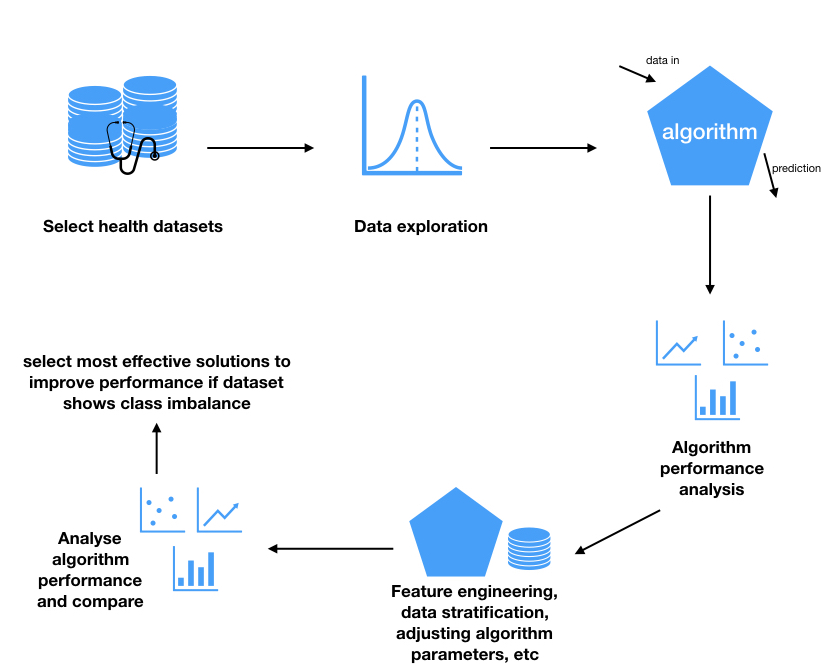
\includegraphics[width=0.8\textwidth]{ThesisTemplate/usingLatex/images/Chapter3Figures001.jpeg}
    \caption{Schematic of the experimental design of the study.}
    \label{fig:expDesign}
\end{figure}

\section{Dataset Choice and Preliminary Exploration}
\subsection{Datasets}
\subsubsection{How were the dataset chosen?}
The Kaggle repository of datasets (https://www.kaggle.com/datasets) was searched for datasets with the tags "healthcare", "health", "oncology and cancer" and "health sciences".
This search returned 223 datasets. Genomic/proteomic datasets were discarded as they are best suited to clustering tasks. Datasets where classification tasks could be carried out were kept and further examined.
A total of 9 datasets were retained for use in the analysis.

\subsubsection{Brief Overview of the datasets}
The datasets chosen for the analaysis were:
\begin{itemize}
    \item Breast Cancer Wisconsin Data Set\footnote{https://www.kaggle.com/uciml/breast-cancer-wisconsin-data}  
    \item Indian Liver Patient Records\footnote{https://www.kaggle.com/uciml/indian-liver-patient-records} 
    \item MRI and Alzheimers \footnote{https://www.kaggle.com/jboysen/mri-and-alzheimers\#oasis\_longitudinal.csv}
    \item Pima Indian dataset\footnote{https://www.kaggle.com/uciml/pima-indians-diabetes-database} 
    \item Cervical Cancer Risk Classification\footnote{https://www.kaggle.com/loveall/cervical-cancer-risk-classification  }
    \item Lower back pain symptom dataset\footnote{ https://www.kaggle.com/sammy123/lower-back-pain-symptoms-dataset}
    \item Heart Attack Prediction\footnote{https://www.kaggle.com/imnikhilanand/heart-attack-prediction}
    \item Autism Screening\footnote{https://www.kaggle.com/faizunnabi/autism-screening/home} 
    \item Fertility dataset\footnote{https://www.kaggle.com/gabbygab/fertility-data-set} 
    
   
\end{itemize}

All 9 datasets allow classification tasks to be carried out, most of them on a binary basis.

\subsection{Class distribution of the datasets}
Table 3.1 sums up the class distribution for the datasets chosen. The class distribution is written in the format HealthyValues - OutcomeValues.
As can be seen from the table, not all datasets have similar class distribution, though most of the selected ones have a 25-25\% of the Outcome class apart from the Autism set and the cervical cancer set which have less than 10\% of the data representing the target class. \newline This range of class distribution will provide interesting case studies to compare the effect of class distribution on the performance of various algorithms. It could also be possible to artificially manipulate the testing data after the split of data by removing instances of the target class so as to mimic real world incidence of the conditions represented in the datasets. In doing so, the performance of various algorithms could be measured on testing sets that are more realistic.

\begin{table}
\begin{tabular}{ p{4.5cm}p{1.5cm} p{1.5cm}  p{2 cm} p{1.5cm}}
 \hline
 \multicolumn{5}{c}{Datasets} \\
 \hline
 \hline
 \rowcolor{LightCyan}
 Dataset Name & Instances & Columns & Class Distribution & \% Minority Class \\
 \hline
 Breast Cancer Wisconsin Data Set& 569 & 32 & 
357-212 & 37.0\\
Indian Liver Patient Records&  583 & 11  & 416-167 & 28.0 \\
Pima Indian dataset& 768 & 9  & 503-265 & 34.0 \\
Cervical Cancer Risk Classification & 858 &  36 & 802-56 & 6.52\\
Lower back pain symptom dataset & 310 & 13  & 101-209 & 67.4\\
Heart Attack Prediction & 294 & 14  & 188-106 & 36.0\\
Autism Screening&704 & 21 &514-90 & 1.2 \\
Fertility dataset&100  & 10 & 89-11 & 11.0\\
\hline
\end{tabular}
\caption{Summary of datasets chosen for the analysis}
\label{tab:1}
\end{table}


\section{Choice of algorithms used in evaluation}
\subsection{Quick overview of algorithms}
This works focuses on supervised learning classification tasks. Several supervised machine learning algorithms have shown promises in computer-aided diagnostic (CAD) \citep{Dua:2014dz}:
\begin{itemize}
    \item decision trees (DT) such as Random Forest are easy to comprehend and relatively easy to implement but are challenging to apply to non linear problems \citep{Gray:2013eh}
    \item support vector machine \citep{Naraei:ct}
    \item k-NN \citep{Liu:2011dz}
    \item Bayesian models \citep{Dangare:ut}
\end{itemize}

\subsection{Reasons for choosing those algorithms}
The algorithms listed above have demonstrated high performance in classifying tasks on healthcare data, even in the case of imbalanced datasets \citep{Dua:2014dz}. They also utilise different mathematical approaches to classification and therefore are expected to behave differently from one another.



\section{Proposed avenues of exploration}
\subsection{Overview of typical methods to address class imbalance}
The class imbalance problem was discussed in chapter 2 along with some of the techniques used to compensate for its effects. These techniques are discussed here further and can be separated in data-level solutions and algorithm-level solutions:
\begin{enumerate}
    \item data-level solutions\citep{Sun:2013it}
    \begin{itemize}
        \item undersampling the prevalent class 
        \item oversampling the minority class
        \item detecting the sub-concepts constituting a class and  oversampling each concept to balance the overall distribution
    \end{itemize}
    \item algorithm level solutions
    the solutions here are highly dependent upon the algorithm and in order o develop an algorithmic solution, knowledge of the classifier learning algorithm and the application domain is necessary as well as a thorough comprehension on why the learning algorithm fails when the class distribution of available data is uneven
    \begin{itemize}
        \item choosing an appropriate inductive bias (e.g. for decision trees, adjusting the pruning technique)
        \item for SVMs, different penalty constants can be used for different classes
    \end{itemize}
    \item cost-sensitive learning\citep{Sun:2013it}
    Cost-sensitive classification considers the varying costs of different misclassification types i.e. various penalties are applied for classifying one class as another. In this situation, the learning aims to minimize high cost misclassifications and the total cost of misclassification.
    Cost-sensitivity can be obtained through:
    \begin{itemize}
        \item weighting the data space
        \item making a classifier cost-sensitive by adjusting parameters to minimize the cost of misclassification
        \item using Bayes Risk Theory to assign each sample to its lowest risk class
    \end{itemize}
\end{enumerate}
\subsection{Testing the Impact of the use of these methods}
\subsubsection{First test the algorithms on the dataset without any modifications}
In the first instance, all of the algorithms will be applied to all of the datasets without parameter optimisation. The performances will be noted (see section 3.5.1). 

\subsubsection{Applying the methods to each datasets and algorithms}


Then the methods discussed in section 3.4.1 will be employed on all of the datasets and the algorithms will be applied to the modified data again so that performance can be compared.\newline In the case of the cost-learning solutions, the parameters of the different classifiers will be adjusted so as to reduce cost of misclassification, before the performance on each dataset is measured again.

\subsubsection{Testing the performance on more realistic datasets}
As an added investigation, the testing data (and potentially training) could be modified to reflect actual incidence of the conditions being observed "in the wild" and the performance of the classifiers could be tested again using the optimised parameters and methods used previously.

\section{Evaluating the performance of classifiers and of correction methods}

\subsection{Metrics for evaluation}  
The metrics to measure the performance of an algorithm have already been reviewed in section 2.2.2. and will be briefly restated here
\subsubsection{Accuracy}
This is the percentage of correct predictions made by a model and is not considered to be a good measure to use when studying highly imbalanced datasets.


\subsubsection{Confusion Matrix}

The confusion matrix describes the complete performance of the model as can be seen on figure. The number of true positives, true negatives, false positives and false negatives are all shown in the confusion matrix.

\begin{figure}[H]
    \centering
    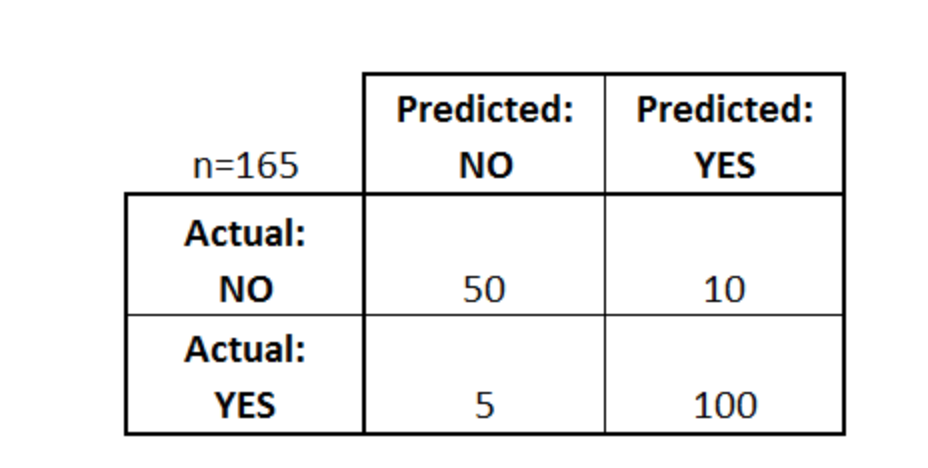
\includegraphics[width=0.5\textwidth]{ThesisTemplate/usingLatex/images/ConfusionMatrix.png}
    \caption{Adapted from Mishra, A., Metrics to Evaluate your Machine Learning Algorithm, TowardsDataScience.com}
    \label{fig:metrics}
\end{figure}

\subsubsection{Area under the curve}
This reflects the probability that the classifier will rank a randomly chosen positive example higher than a randomly chosen negative example. Its value is expressed between 0 and 1 (the closer to 1 the better the performance).


\subsubsection{F1 score}
This measures a test's accuracy and is obtained by calculating the harmonic mean between precision and recall. It reflects the classifier's precision and its robustness.

\subsubsection{Others}
Negative Predictive Value, Calibration and Specificity are also useful measures and may be used in the analysis.

\subsection{Choice of most relevant metrics}
\subsubsection{which metrics will be most helpful in the healthcare context}
In the context of healthcare, it is unlikely that accuracy will be very useful; not only it is a poor metric of performance for imbalanced data but the cost of misclassification in health matters could be extremely high and therefore, a poor metric is not suitable and would be at best indicative prior further analysis.

The other metrics discussed will all be considered and evaluated as to what constitutes the best measure for algorithm performance in this context.

\subsubsection{create a combined metric for this evaluation}
It may be useful to combine several of these metrics to get a more complete picture of how good or how poor the classifier is at identifying its target labels.

\subsection{Comparing performance of algorithms for each dataset before and after applying the methods to compensate for class imbalance}
Once the "baseline" performance of each classifier on the different datasets has been assessed by using the metrics discussed above, the same metrics will be measured on the same combinations of classifiers/data after implementations of the corrective methods. 
The resulting metrics can then be compared and the most effective method(s) can be assessed. It is expected that the methods to be applied will be more or less successful depending on the classifier and on the data rather than improving uniformly across all.

\section{Technical Requirements}
\subsection{Language}
R and Python are the most commonly used languages for data science and analytics. R provides some powerful and user friendly graphs and statistics, therefore making a good visualisation tool. On the other hand python focuses on productivity and code readability.
Python is better choice if the data analytics and machine learning being carried out is closely linked to a development environment, whereas R has been mostly used in the area of statistics and research \citep{Willems:2015wi}.
Since this projects will not be involved in the development of an application or support an application logic, R will be used as it offers a large resource base of libraries and visulation options.

\subsection{Software}

R Studio will be used to write and compile code for this project. Microsoft Excel may also be used to examine some of the raw data as tables. 
None of the datasets are very large and it is not thought that this project will necessitate the use of distributed file systems such as Hadoop.

\section{Discussion of results}
\subsection{Results obtained}
Results of analysis will be collected after each run and analysis will repeated multiple times with the results aggregated so as to avoid variations.
The various settings of each experiment will be carefully recorded so as to be aware of which parameters was used or which way the data was pre-processed prior analysis.

\subsection{Driving factors for the results}
The results will be assessed and discussed so as to determine which combination of parameters, algorithm choice and data processing would produce optimal performance, though this will also be balanced with practical concerns and the various costs and benefits of each factors will be discussed.


\section{Conclusions}

This chapter has outlined the experimental design for this project and in which way the results will be assessed and how will the success of the project be appraised. 
Nine health-related datasets have been chosen from publicly available sources and four algorithms will be used as classifiers on these datasets. The algorithms were chosen based on previous reported performance in the health sector. The different methods (data-level and algorithm-level) that can be applied to correct problems created by heavily imbalanced classes in health data have been discussed and their effects on the performance of the chosen classifiers will be assessed by measuring several performance metrics before and after their use.
The chosen performance metrics (AUC, confusion matrix, F1 score, etc) will be used to determine which methods are the most effective.





